Before going further in this section, we must clarify that the information and figures presented here are merely auxiliary. The dimensionality reduction t-SNE technique was used since it is particularly well suited for the visualization of high-dimensional datasets.

Dimensionality reduction techniques are out of the scope of this report but we'll provide a brief intuition on how t-SNE works. t-SNE attempts to solve the crowding problem. It models each high-dimensional object by a two or three-dimensional point such that similar objects are modeled by nearby points and dissimilar ones by distant points.

Results shown in further figures were using the actual embedded data and in no way intend to replicate or accurately explain the behavior obtained when using the actual high-dimensional dataset but rather provide a good approximation.

All 1593 observations in the semeion-dataset were embedded using t-SNE. Figures \ref{fig:tSNE_0} and \ref{fig:tSNE_234} are rather self-explanatory and interesting differences can be appreciated depending on the weighting function used, particularly in the northwest region of the plots.
\begin{figure}[b]
	\centering
	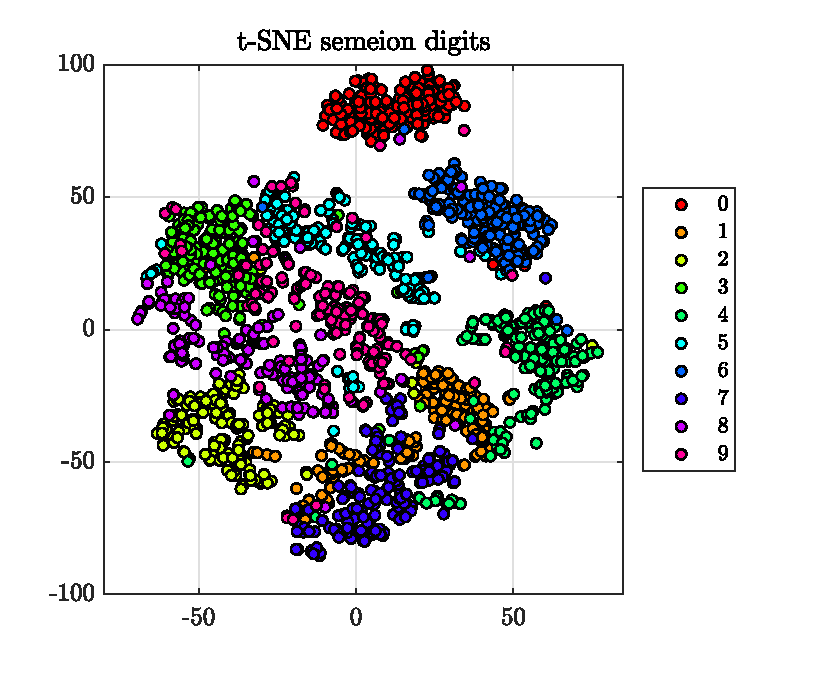
\includegraphics[width=0.45\textwidth, trim={15 15 25 0}, clip]{tSNE_0}
	\caption{Raw t-SNE embedding of semeion-data using euclidean distance}
	\label{fig:tSNE_0}
\end{figure}
%\begin{figure}
%	\centering
%	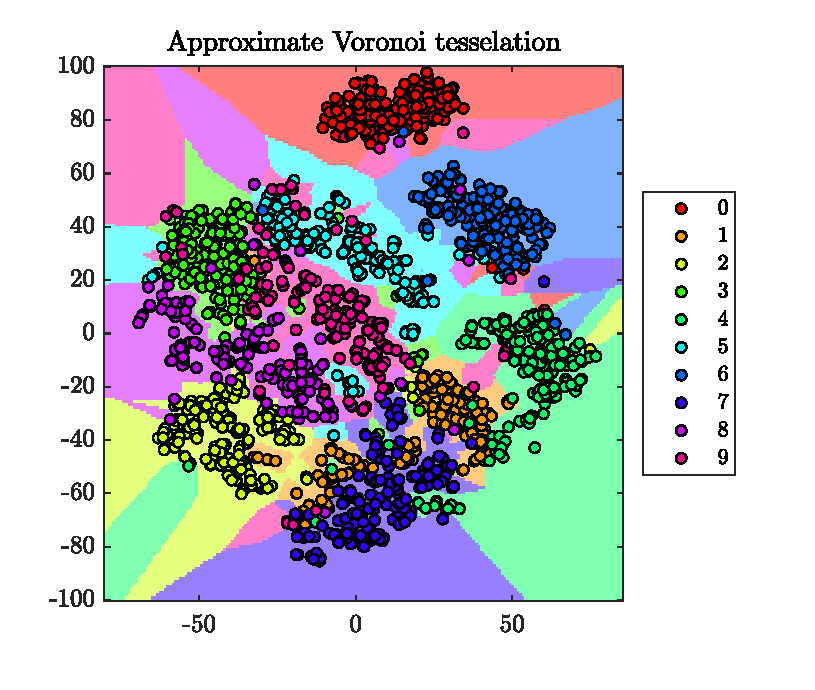
\includegraphics[width=0.45\textwidth]{tSNE_1}
%	\caption{Approximate Voronoi tesselation using 1-NN classification}
%	\label{fig:tSNE_1}
%\end{figure}
\begin{figure}[]
	\centering
	\begin{subfigure}[]{0.45\textwidth}
		\centering
		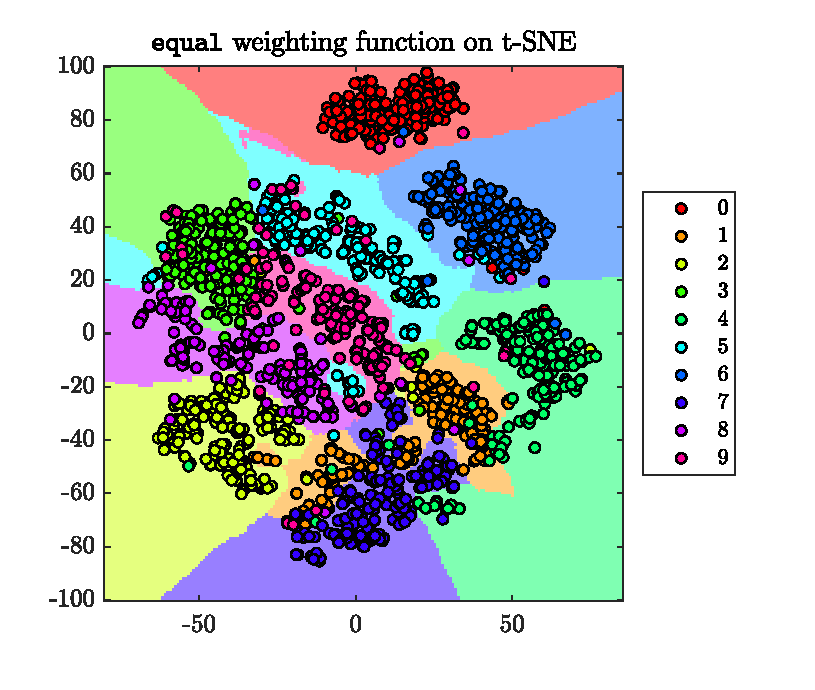
\includegraphics[width=\textwidth, trim={15 15 25 0}, clip]{tSNE_2}
		%\caption{\texttt{equal} weighting function} \vspace*{2mm}
		% \label{fig:gull}
	\end{subfigure}
	%add desired spacing between images, e. g. ~, \quad, \qquad, \hfill etc. 
	%(or a blank line to force the subfigure onto a new line)
	\begin{subfigure}[]{0.45\textwidth}
		\centering
		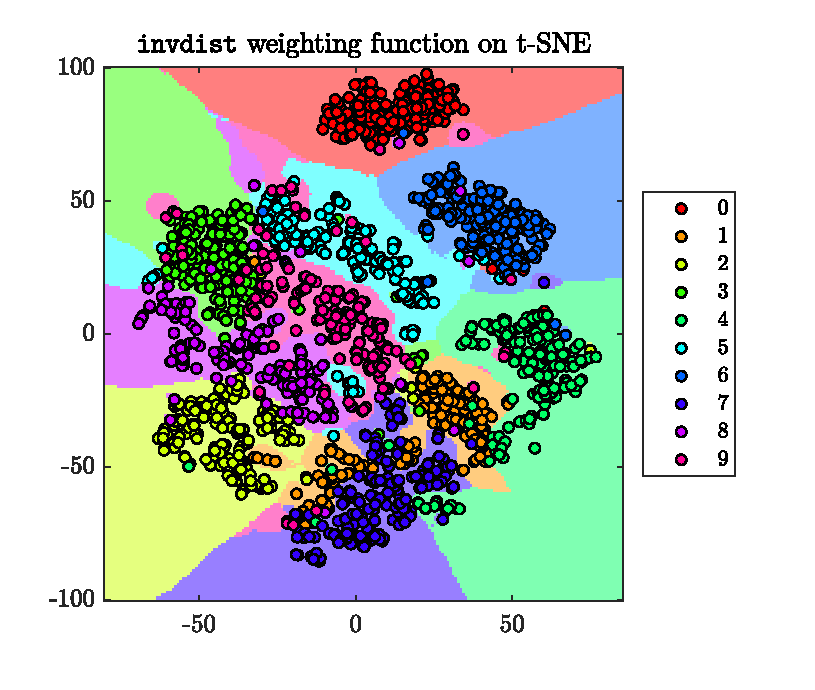
\includegraphics[width=\textwidth, trim={15 15 25 0}, clip]{tSNE_3}
		%\caption{\texttt{invdist} weighting function} \vspace*{2mm}
		% \label{fig:gull}
	\end{subfigure}
	\begin{subfigure}[]{0.45\textwidth}
		\centering
		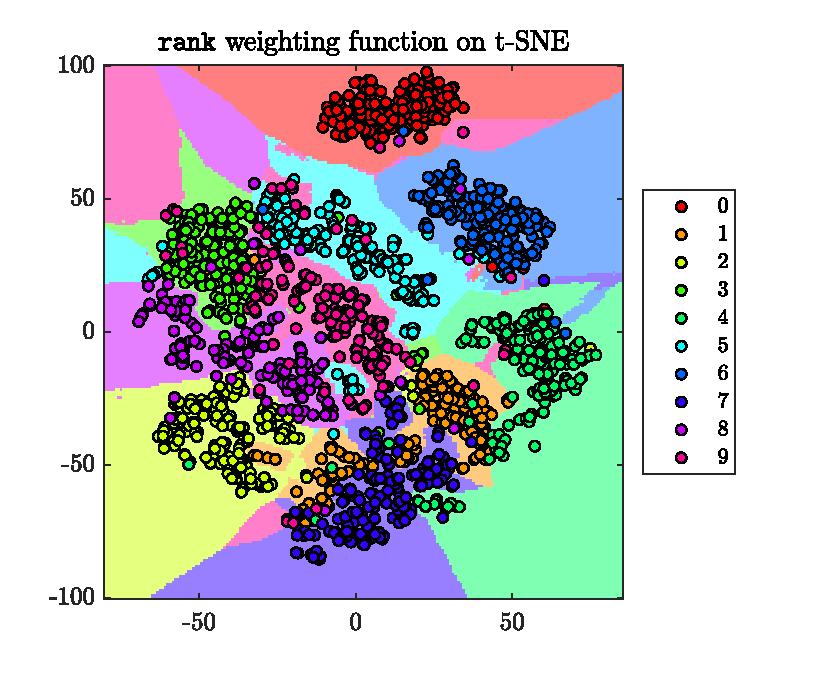
\includegraphics[width=\textwidth, trim={15 15 25 0}, clip]{tSNE_4}
		%\caption{\texttt{rank} weighting function} \vspace*{2mm}
		% \label{fig:tiger}
	\end{subfigure}
	\caption{Approximate Voronoi tesselations using 10-NN classification. Each new point will be classified according to the color of the region it lies in.}
	\label{fig:tSNE_234}
\end{figure}